\documentclass[conference]{IEEEtran}
\IEEEoverridecommandlockouts
% The preceding line is only needed to identify funding in the first footnote. If that is unneeded, please comment it out.
\usepackage{cite}
\usepackage{amsmath,amssymb,amsfonts}
\usepackage{algorithmic}
\usepackage{graphicx}
\usepackage{textcomp}
\usepackage{xcolor}
\def\BibTeX{{\rm B\kern-.05em{\sc i\kern-.025em b}\kern-.08em
    T\kern-.1667em\lower.7ex\hbox{E}\kern-.125emX}}

\ifCLASSINFOpdf
\else
    \usepackage[dvips]{graphicx}
\fi
\usepackage{url}
\usepackage{listings}
% \usepackage[margin=1in]{geometry}
\usepackage{amsmath,amsthm,amssymb}
\usepackage{amsmath,amsthm,amssymb}
\usepackage[spanish]{babel} %Castellanización
\usepackage[T1]{fontenc} %escribe lo del teclado
\usepackage[utf8]{inputenc} %Reconoce algunos símbolos
\usepackage{lmodern} %optimiza algunas fuentes
\usepackage{blkarray}
\graphicspath{ {images/} }
\usepackage{hyperref} % Uso de links

\newcommand{\N}{\mathbb{N}}
\newcommand{\Z}{\mathbb{Z}}
\usepackage{float}
\newenvironment{theorem}[2][Theorem]{\begin{trivlist}
\item[\hskip \labelsep {\bfseries #1}\hskip \labelsep {\bfseries #2.}]}{\end{trivlist}}
\newenvironment{lemma}[2][Lemma]{\begin{trivlist}
\item[\hskip \labelsep {\bfseries #1}\hskip \labelsep {\bfseries #2.}]}{\end{trivlist}}
\newenvironment{exercise}[2][Exercise]{\begin{trivlist}
\item[\hskip \labelsep {\bfseries #1}\hskip \labelsep {\bfseries #2.}]}{\end{trivlist}}
\newenvironment{problem}[2][Problem]{\begin{trivlist}
\item[\hskip \labelsep {\bfseries #1}\hskip \labelsep {\bfseries #2.}]}{\end{trivlist}}
\newenvironment{question}[2][Question]{\begin{trivlist}
\item[\hskip \labelsep {\bfseries #1}\hskip \labelsep {\bfseries #2.}]}{\end{trivlist}}
\newenvironment{corollary}[2][Corollary]{\begin{trivlist}
\item[\hskip \labelsep {\bfseries #1}\hskip \labelsep {\bfseries #2.}]}{\end{trivlist}}
\newcommand*{\defeq}{\stackrel{\text{def}}{=}}
\newenvironment{solution}{\begin{proof}[Solution]}{\end{proof}}
\hyphenation{op-tical net-works semi-conduc-tor}

\newcommand{\argmax}{\operatornamewithlimits{argmax}}


\usepackage[ruled,vlined]{algorithm2e}

\begin{document}

\title{Tarea 3. Optimización }

\author{\IEEEauthorblockN{Oscar Esaú Peralta Rosales}
\IEEEauthorblockA{\textit{Maestría en Computación} \\
\textit{Centro de Investigación en Matemáticas}}
}

\maketitle

\begin{abstract}
Se presenta una solución al problema

$$x^* = \underset{x \in \mathcal{R}^n}{\mathrm{argmin}} f(x)$$

con
$f(x) = \sum_{i=1}^{n} (x_i-y_i)^2 + \lambda \sum_{i=1}^{n-1} (x_{i+1} - x_i)^2$\\

usando dos algoritmos, Descenso de Gradiente y el Método de Newton. Para
problemas cuadráticos como el presentado aquí el Método de Newton converge
en una sola iteración echo mostrado en los cuadros comparativos del algoritmo.
En la sección Apéndice (V-A) se muestran los resultados a tres problemas con respecto
a temas de los algoritmos de búsqueda en linea aquí planteados.

\end{abstract}

\begin{IEEEkeywords}
Descenso de gradiente, Método de Newton
\end{IEEEkeywords}

\section{Introduction}

El método de Descenso de Gradiente es uno de los métodos de búsqueda en linea que
nos permite resolver problemas de optimización al ayudarnos a encontrar máximos
o mínimos dentro de funciones. La idea general detrás de este método es sencilla;
dado un punto solución inicial $x_0$ a una función $f$ (tomada al azar o una aproximación cualquiera) podemos
encontrar otra solución que mejore nuestra evaluación (en términos de maximizar
o minimizar) en $f$, con ayuda de el gradiente en ese punto. El gradiente nos
indica la dirección de máximo crecimiento (existen más direcciones de crecimiento
pero esta es la máxima) en la función, por tanto, moverse ese dicha dirección o
en sentido contrario nos permite encontrar máximos o mínimos (No tenemos
garantizado la convergencia a un mínimo o máximo global). En general la selección
de nuestro nuevo punto solucion se realiza mediante (para minimización)
$x_{k+1} = x_k - \alpha \nabla f(x_k)$\\

El Método de Newton considera la actualización en cada iteración como
$x_{k+1} = x_k - \nabla^2 f(x_k) \nabla f(x_k)$, sin embargo la matriz Hessiana
$\nabla^2f(x_k)$ no siempre es definida positiva y $\nabla^2 f(x_k) \nabla f(x_k)$
podría no ser una dirección de descenso. Para resolver este problema se busca
obtener una nueva matriz a partir de la Hessiana tal que ésta si sea definida
positiva, ie. $B_k = \nabla^2f(x_k) + E_k$ para ello podemos construir
$E_k = \tau_kI$ tal que $\tau$ nos asugure que $B_k$ se definida positiva el cual
podemos elegir como el valor propio más pequeño del Hessiano, la implementación
aquí realizada computa ese valor con ayuda de la factorizando de Cholesky
Modificado.

\section{Métodología}

Cómo se menciona anteriormente el problema a resolver consiste en encontrar
$$
	x^* = \underset{x \in \mathcal{R}^n}{\mathrm{argmin}} f(x)
$$

donde $f(x) = \sum_{i=1}^{n} (x_i-y_i)^2 + \lambda \sum_{i=1}^{n-1} (x_{i+1} - x_i)^2$
usando Descenso de Gradiente y Métodos de Newton,
considerando $\lambda \in \{1, 100, 1000\}$ \\

Ambos métodos descritos arriba requieren para su implementación el cálculo
del gradiente y el hessiano de la función, las cuales se muestran en el
apéndice (V-C).

Cabe notar que en este caso la matriz Hessiana es constante con respecto a el
$x_k$ actual calculado en cada iteración y solo depende del parámetro $\lambda$
elegido.

A continuación se describen de manera general la implementación para los métodos
de Descenso de Gradiente y Método de Newton.

\begin{algorithm}[]
	\SetAlgoLined
	\KwResult{$x^*$}
	x <- Inicializar \\
	$\alpha$ <- Inicializar \\
	\While{Criterio de parada no se cumpla}{
		$\alpha$ <- Actualizar $\alpha$\\
	  	x = x + $\alpha$ - $\nabla$ f(x)\\
	 }
	 \caption{Descenso de Gradiente}
\end{algorithm}
\begin{algorithm}[]
	\SetAlgoLined
	\KwResult{$x^*$}
	x <- Inicializar \\
	$\alpha$ <- Inicializar \\
	\While{Criterio de parada no se cumpla}{
		$B = \nabla^2f(x) $ \\
		\If{B no es semidefinida positiva}{
			$B = B + min_{eigvalue}(B)$ \\
		}
	  	x = x - $\alpha$ * $B^{-1}$ $\nabla$ f(x)\\
	 }
	 \caption{Método de Newton}
\end{algorithm}

En los dos métodos se usaron 3 criterios de paro:

\begin{itemize}
	\item $\frac{||x_{k+1} - x_{k}||}{max(||x_k||, 1)} < \tau_1$
	\item $\frac{abs(f(x_{k+1}) - f(x_{k}))}{max(abs(f(x_k)), 1)} < \tau_2$
	\item $||\nabla f(x_k)|| < \tau_3$
\end{itemize}

Donde las parámetros a $\tau_1$, $\tau_2$ y $\tau_3$ son elegidos con un valor
aproximado a $1x10^{-12}$. \\

Para el cálculo de $\alpha_k$ usado como el tamaño de para al k-ésima iteración
se realizó de de 3 formas;

\begin{itemize}
	\item Paso Fijo
	\item Paso Autoadaptable con $alpha_k = \frac{g_k^tg_k}{g_k^tHg_k}$, $g_k$ como el gradiente y $H$ el Hessiano en la k-ésima iteración
	\item Método de Backtracking
\end{itemize}

Conservando al final solo el paso Autoadaptable para el Método de
Gradiente y el paso fijo con $\alpha=1$ para el Método de Newton debido a que
se estos se comportaron mejor durante las pruebas y cuyo resultados se muestran
en la siguiente sección.

La actualización del tamaño de paso mediante el \textit{Backtracking} se realiza
de la siguiente mediante el algoritmo listado en el apéndice (V-B).

\section{Resultados}

Las figuras \ref{fignl1}, \ref{fignl100} y \ref{fignl1000} muestran los resultados
obtenidos al minimizar la función $f$. Observemos que en la primer sumatoria
$\sum_{i=1}^{n} (x_i , y_i)^2$ buscamos minimizar la diferencia entre el $Y$ y $X$
así como se puede observar en la figura \ref{fignl1} la aproximación de $x_i$ a
cada $y_i$ es muy buena. Mientras $\lambda$ crece la aproximación de los valores
de cada $y_i$ es menor, debido al castigo por la ponderación que provoca la
segunda sumatoria, así entonces un efecto de suavizado aparece en las figuras
\ref{fignl100} y \ref{fignl1000}.


\begin{figure}[htbp]
	\centerline{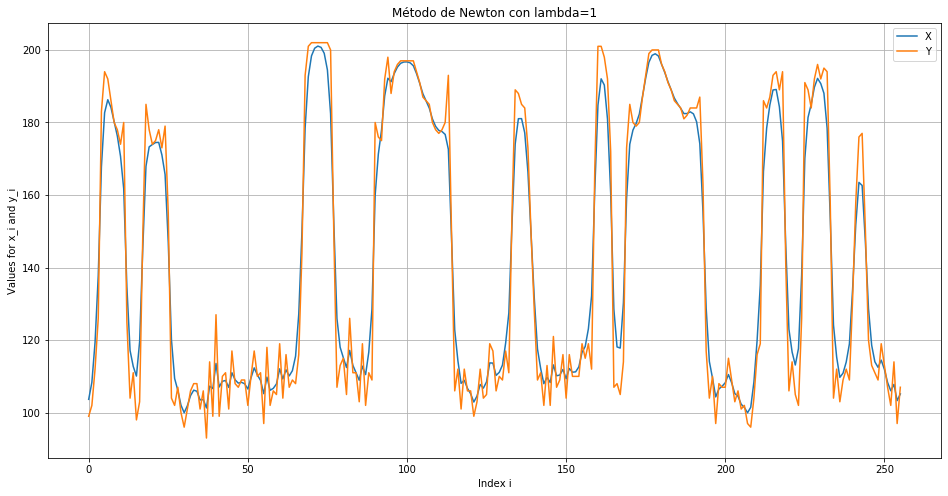
\includegraphics[scale=0.26]{nl1.png}}
	\caption{Obtención del minimizador para la función con $\lambda=1$, se observa una buena aproximación sobre los la serie formada por el vector Y.}
	\label{fignl1}
\end{figure}

\begin{figure}[htbp]
	\centerline{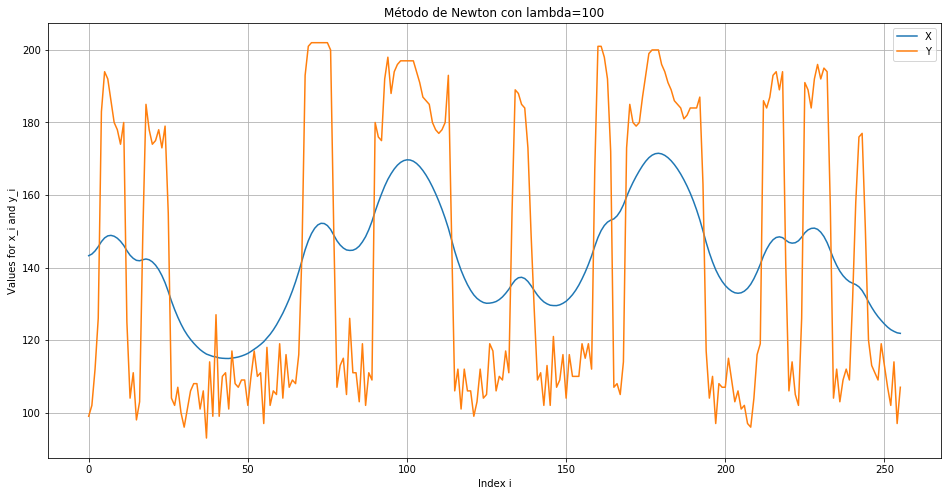
\includegraphics[scale=0.26]{nl100.png}}
	\caption{Obtención del minimizador para la función con $\lambda=100$, se observa un suavizado provocado por el contribución de $\lambda$.}
	\label{fignl100}
\end{figure}

\begin{figure}[htbp]
	\centerline{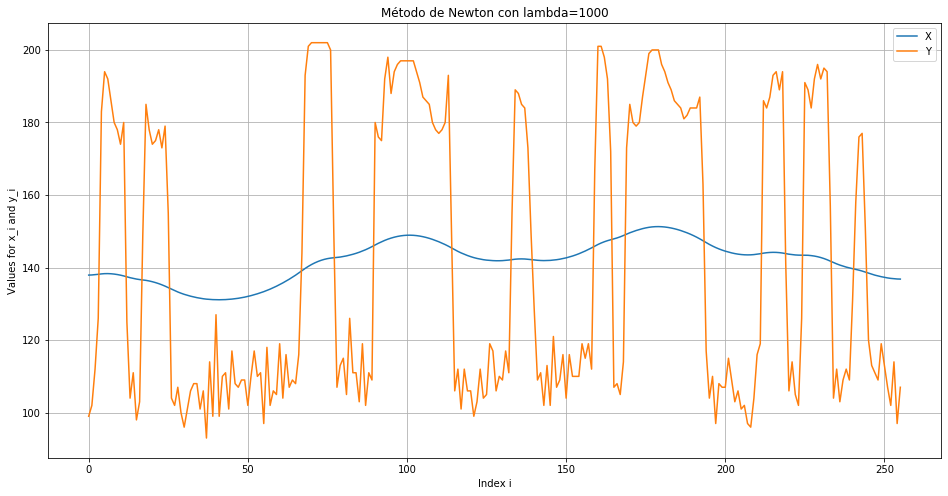
\includegraphics[scale=0.26]{nl1000.png}}
	\caption{Obtención del minimizador para la función con $\lambda=1000$, el suavizado de los la serie de los valores de Y es más intenso.}
	\label{fignl1000}
\end{figure}

Las graficas obtenidas mediante el método de Descenso de Gradiente se muestran
en el apéndice (V-D).

\begin{table}[htbp]
	\caption{Método de Newton con $\alpha=1$}
	\begin{center}
		\begin{tabular}{|c|c|c|c|}
			\hline
			\textbf{\textit{$\lambda$}}& \textbf{\textit{Iteraciones}}& \textbf{\textit{Tiempo}}& \textbf{\textit{Error}} \\
			\hline
			1& 2 & 0.0908 & 1.00638198e-16 \\
			100& 2 & 0.0941 & 3.25256674e-15 \\
			1000& 2 & 0.0959 & 6.27304335e-15 \\
			\hline
			\multicolumn{4}{l}{}
		\end{tabular}
		\label{tabn}
	\end{center}
\end{table}

Como se observa en los resultados de la tabla \ref{tabn} el Método de Newton la
convergencia la alcanza en la primer iteración (Nótese que se necesita al menos
dos iteraciones para verificar convergencia), comprobando así la convergencia en
un solo paso pára problemas cuadráticos.

\begin{table}[htbp]
	\caption{Descenso de Gradiente con $\alpha$ Autoadaptable}
	\begin{center}
		\begin{tabular}{|c|c|c|c|}
			\hline
			\textbf{\textit{$\lambda$}}& \textbf{\textit{Iteraciones}}& \textbf{\textit{Tiempo}}& \textbf{\textit{Error}} \\
			\hline
			1& 32 & 0.0514 & 9.90900042e-13 \\
			100& 2376 & 3.774 & 9.98161882e-13 \\
			1000& 19135 & 25.155 & 9.99757740e-13 \\
			\hline
		\end{tabular}
		\label{tabg1}
	\end{center}
\end{table}
\begin{table}[htbp]
	\caption{Descenso de Gradiente con $\alpha$ Fijo}
	\begin{center}
		\begin{tabular}{|c|c|c|c|c|}
			\hline
			\textbf{\textit{$\lambda$}}& $\alpha$ &\textbf{\textit{Iteraciones}}& \textbf{\textit{Tiempo}}& \textbf{\textit{Error}} \\
			\hline
			1& 0.017 & 38 & 0.0376 & 8.50063163e-13 \\
			100& 0.0024 & 2518 & 1.161 & 9.96273014e-13 \\
			1000& 0.0001 & 47337 & 24.396 & 9.99757738e-13 \\
			\hline
		\end{tabular}
		\label{tabg2}
	\end{center}
\end{table}
\begin{table}[htbp]
	\caption{Descenso de Gradiente con $\alpha$ mediante Backtracking}
	\begin{center}
		\begin{tabular}{|c|c|c|c|c|}
			\hline
			\textbf{\textit{$\lambda$}}& $\alpha$ &\textbf{\textit{Iteraciones}}& \textbf{\textit{Tiempo}}& \textbf{\textit{Error}} \\
			\hline
			1 & 0.017 & 38 & 0.0368 & 8.50063163e-13 \\
			100 & 0.0024 & 2518 & 1.409 & 9.96273014e-13 \\
			1000 & 0.0001 & 47337 & 27.247 & 9.99757738e-13 \\
			\hline
			\multicolumn{4}{l}{Se usó $\rho=0.001$ y  $c1=1e-14$}
		\end{tabular}
		\label{tabg3}
	\end{center}
\end{table}

Las tablas \ref{tabg1}, \ref{tabg2}, \ref{tabg3} muestran los resultados para el
algoritmo de Descenso de Gradiente. La convergencia por este método requiere más
iteraciones y mientras el valor de $\lambda$ aunmenta converge más lento.
Los mejores tiempos y número de iteraciones se obtuvieron con $\alpha$
Autoadaptable.

\section{Conclusiones}

Para la solución de este problema sin duda el mejor algoritmo fue el Método de
Newton, el cual converge con una sola iteración, tal como teóricamente se habia
demostrado en clase. Con el algoritmo de Descenso de Gradiente también se
obtuvieron muy buenos resultados (con errores de en rango de $1e^{-13}$) pero
se requirieron más iteraciones para converger y estas crecen mientras se escoga
una $\lambda$ más grande. \\

Como vimos, el efecto de elegir un valor de $\lambda$ mayor repercute directamente
en la eficiencia del Algoritmo de método de Descenso de Gradiente pero no es el
único efecto que realiza, puesto como se observó en los gráficos anteriores,
tiene un efecto en la aproximación a cada valor $y_i$ suavizando el resultado final.\\

Usando el método de actualización de paso con Backtracking solo se logró hacer
simil al de paso fijo, por tanto ambas tablas muestran resultados parecidos.

Cómo un la matriz Hessiana obtenida para los valores de $\lambda$ es definida
positiva la actualización de dicha matriz mediante el algoritmo de la
Factorización de Cholesky para encontrar en el valor propio más pequeño
no fue necesario, más sin embargo su implementación se encuentra en el código
adjunto a este reporte.

\section{Apéndice}

\subsection{Problemas}

\subsubsection*{1}

Considera la función $f(x_1, x_2) = (x_1 + x_2^2)^2$. En el punto $x^T = [1, 0]$
consideramos la dirección de búsqueda $p^T = [-1, 1]$. Muestra que $p$ es una
dirección de descenso y encuentra todos los minizadores de la función. \\

\textbf{Solución}

Sabemos que un vector $p$ es una dirección de descenso si $\nabla^T f(x) p < 0$,
para algún vector $x$. El gradiente de $f$ está dado por
$\nabla f(x_1, x_2) = [2(x_1+x_2^2)\ \ 4(x_1 + x_2^2)x_2]^T$, evaluando en el punto
$x^T = [1, 0]$ tenemos que $\nabla f(1, 0) = [2\ \ 0]^T$ entonces
$\nabla^T f(1, 0) p =  [2\ \ 0]\ [-1\ \ 0]^T = -2 < 0$ y así $p$ es una
dirección de descenso. \

Para encontrar todos los puntos que minimizan la función, procedemos a
encontrar aquellos que son puntos estacionarios igualando el gradiente a cero y
resolviendo el sistema de ecuaciones generado.

$$
\nabla f(x_1, x_2) =
\begin{pmatrix}
	2 x_1 + 2 x_2^2 \\
	4 x_1x_2 + 4 x_2^2 \\
\end{pmatrix} =
\begin{pmatrix}
    0 \\
    0 \\
\end{pmatrix}
$$

La solución al sistema anterior es $x_! = -x_2^2$, es decir todos aquellos puntos
de la forma $(-a^2, a),\ a \in \mathcal{R}$. Un punto es un minimizador si la matriz
Hessiana de $f$ asociada al punto es definida o semidefinida positiva. La matriz
Hessiana de $f$ está dada por

$$
\nabla^2 f(x_1, x_2) =
\begin{pmatrix}
	2 && 4x_2 \\
	4x_2 && 4x_1 + 12x_2^2 \\
\end{pmatrix}
$$

Para saber si es definida o semidefinida positiva evaluamos un punto de la forma
$(-x_2^2, x_2)$ y calculamos su determinante.

$$
det
\begin{pmatrix}
	2 && 4x_2 \\
	4x_2 && -4x_2^2 + 12x_2^2 \\
\end{pmatrix} =
16x_2^2 - 16x_2^2 = 0
$$

Como el determinante es cero, no tenemos demasiada información para tomar una desición.
Sin embargo, notemos que siempre $f(x_1, x_2) \ge 0$ para cualquier punto $[x_1, x_2]$
y en especial para los puntos de la forma $(-x_2^2, x_2)$ la función $f$ alcanza el mínimo
valor posible; cero. Así todos los puntos de la forma $(-x_2^2, x_2)$ minimiza a $f$.
Por inspección podemos ver el comportamiento de la función en \ref{fig1} para
corroborar visualmente que efectivamente esa serie de puntos son minimizadores.\\

\begin{figure}[htbp]
	\centerline{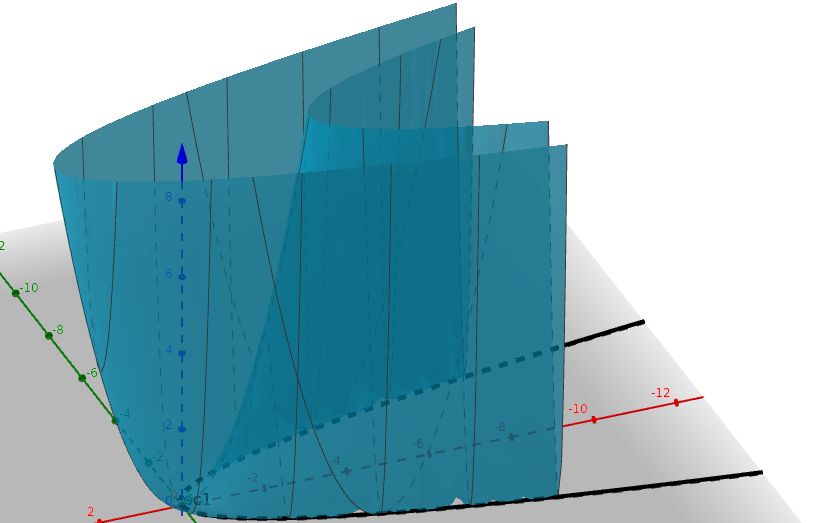
\includegraphics[scale=0.3]{fig1.png}}
	\caption{Para problema 1. De azul la función $f(x_1. x_2) = (x_1, x_2^2)^2$,
	de negro todos los puntos de la forma ($-x_2^2, x_2$) que minimizan a $f$.}
	\label{fig1}
\end{figure}

\subsubsection*{2}

Encuentra todos los valores del parámetro $a$ tal que $[1, 0]^T$ es un minizador o
maximizador de la función $f(x_1, x_2) = a^3x_1e^{x_2} + 2a^2log(x_1 + x_2) - (a+2) + 8ax_2 + 16x_1x_2$.
\\

\textbf{Solución}

Cómo el punto $[1, 0]^T$ es un minimizador o maximizador de $f$ entonces $\nabla f(1, 0) = [0 , 0]$.
Obtenemos primeramente el gradiente de $f$ el cual es
$\nabla f(x_1, X_2) = [a^3e^{x_2} + \frac{2a^2}{x_1 + x_2} - (a + 2) + 16x_2 \ \ \ a^3e^{x_2} + \frac{2a^2}{x_1 + x_2} + 8a + 16x_1]^T$
(asumiendo que $log$ es logaritmo natural). Sustiyendo el punto $[1, 0]^T$ obtenemos el
sistema de ecuaciones $a^3 + 2a - a - 2 = 0$ y $a^3 + 2a + 8a + 16 = 0$, factorizando
tenemos $(a+2)(a^2-1) = 0$ y $(a+2)(a^2-8) = 0$. Así, para solo para $a = -2$ se cumple
que $\nabla f(1, 0) = [0 , 0]$. \\

Evaluamos $a=-2$ el el Hessiano de $f$ para comprobar que es un minimizador o un maximizador,
donde el Hessiano está dado por

$$
\nabla^2 f =
\begin{pmatrix}
	- \frac{2a^2}{(x_1 + x_2)^2} && a^3e^{x_2} - \frac{2a^2}{(x_1 + x_2)^2} + 16 \\
	a^3 e^{x_2} - \frac{2a^2}{(x_1 + x_2)^2} + 16 && a^3 x_1 e^{x_2} - \frac{2a^2}{(x_1 + x_2)^2} \\
\end{pmatrix}
$$

Evaluando en el punto punto $[1, 0]^T$ y con $a=-2$

$$
\begin{pmatrix}
	- 2a^2 && a^3 - 2a^2 + 16 \\
	a^3 - 2a^2 + 16 && a^3 - 2a^2 \\
\end{pmatrix}
=
\begin{pmatrix}
	-8 && 0 \\
	0 && -16 \\
\end{pmatrix}
$$

Podemos ver que la matriz Hessiana es definida negativa puesto que los sus
valores propios son $\lambda = -8$ y $\lambda = -16$ por tanto para $a=-2$ el
punto $[1, 0]^T$ es un maximizador de $f$. \\


\subsubsection*{3}

Sea $f: \mathcal{R}^n \rightarrow \mathcal{R}$ dado por $f(x) = \frac{1}{2}x^TQx - b^Tx$
con $b \in \mathcal{R}^n$ y $Q \in \mathcal{R}^{nxn}$ una matriz real simetrica y
definida positiva. Considera el algoritmo $x^{k+1} = x^k - \beta \alpha_k \nabla f(x^k)$
donde $\alpha_k = \frac{\nabla f(x^k)^T \nabla f(x^k) }{\nabla f(x^k)^T Q \nabla f(x^k)}$.
Muestra que $\{x^k\}$ converge a $x^* = Q^{-1}b$ para cualquier punto inicial $x^0$
si y solo si $0 < \beta < 2$. \\

\textbf{Solución}

Notemos que $\nabla f(x) = Qx_k - b$ y $x^*$ minimiza la función y como es
solución de $Qx^* - b = 0$  converge a $Q^{-1}b$. Por otro lado, dada una
secuencia de  $\{x^k\}$ resultante de la actualización
$x^{k+1} = x^{k} - \alpha_k g_k$, con $g_k$ como el gradiente en la k-ésima
iteración del algoritmo de descenso de gradiente y sea
$\gamma_k = \alpha_k \frac{g_k^tQg_k}{g_k^tQ^{-1}g_k} \big(2\frac{g_k^tg_k}{g_k^tQg_k} - \alpha_k \big)$
con $\gamma_k > 0$ para todo $k$, entonces, $\{x^k\}$ converge a $x^*$ para
cualquier punto inicial $x^0$ si y solo si
$\sum_{k=1}^{\infty} \gamma_k = \infty$. \

En particular para la actualización anterior y un tamaño de paso $\alpha_k = \frac{g^t_kg_k}{g^t_kQg_k}$
la secuencia $\{x^k\}$ converge a $x^*$ para cualquier condición inicial $x^0$, en otras paralabras
se cumple que $\sum_{k=1}^{\infty} \gamma_k = \infty$. \

Ahora, sea $\alpha\prime_k = \beta \alpha_k = \beta \frac{g^t_kg_k}{g^t_kQg_k}$, luego \

$\gamma\prime_k = \beta \frac{g^t_kg_k}{g^t_kQg_k} \frac{g_k^tQg_k}{g_k^tQ^{-1}g_k} \big(2\frac{g_k^tg_k}{g_k^tQg_k} - \beta \frac{g^t_kg_k}{g^t_kQg_k} \big)$ \

$\gamma\prime_k = \beta \frac{g^t_kg_k}{g^t_kQg_k} \frac{g_k^tQg_k}{g_k^tQ^{-1}g_k} \big((2 - \beta) \frac{g^t_kg_k}{g^t_kQg_k} \big)$ \

$\gamma\prime_k = \frac{g^t_kg_k}{g^t_kQg_k} \frac{g^t_kg_k}{g^t_kQg_k} (2 - \beta) \beta$ \

$\gamma\prime_k = \gamma_k (2 - \beta) \beta$ \

Por la desigualdad de Rayleigh sabemos que
$\frac{a}{A} \le \gamma_k \le \frac{A}{a}$, donde $a$ y $A$ son los valores
propios (siempre positivos) de $Q$. Entonces para
$\frac{a}{A} (2 - \beta) \beta \le \gamma_k (2 - \beta) \beta \le \frac{A}{a} (2 - \beta) \beta $
se cumple que
$\sum_{k=1}^{\infty} \gamma\prime_k = \sum_{k=1}^{\infty} \gamma_k (2 - \beta) \beta = \infty$
solo para $\beta \in (0, 2)$, puesto que como $\gamma > 0$ y con $\beta \ge 2$
o $\beta \le 0$ el producto $\gamma_k (2 - \beta) \beta$ es $\le 0$. \\


\subsection{Algoritmo para actualización de tamaño de paso Backtracking}

\begin{algorithm}[]
	\SetAlgoLined
	\KwResult{$\alpha$}
	$\alpha$ <- Inicializar \\
	$\rho$ <- Inicializar \\
	$c1$ <- Inicializar \\
	\While{$f(x_k - \alpha * g_k) > f(x_k) + c1 * g_k^T g_k$}{
		$\alpha = \alpha * \rho$ \\
	 }
	 \caption{Método de Backtracking para tamaño de paso}
\end{algorithm}


\subsection{Gradiente y Hessiano de la función a minimizar}

$$
f(x) = \sum_{i=1}^{n} (x_i-y_i)^2 + \lambda \sum_{i=1}^{n-1} (x_{i+1} - x_i)^2
$$

$$\nabla f = $$
$$
\begin{pmatrix}
	2(x_0-y_0) - 2\lambda(x_1-x_0) \\
	2(x_1-y_1) - 2\lambda(x_2-x_1) + 2\lambda (x_1 - x_0) \\
	2(x_2-y_2) - 2\lambda(x_3-x_2) + 2\lambda (x_2 - x_1) \\
	\vdots \\
	2(x_{n-2}-y_{n-2}) - 2\lambda(x_{n-1}-x_{n-2}) + 2\lambda (x_{n-2} - x_{n-3}) \\
	2(x_{n-1}-y_{n-1}) - 2\lambda(x_{n}-x_{n-1}) + 2\lambda (x_{n-1} - x_{n-2}) \\
	2(x_{n}-y_{n}) + 2\lambda (x_{n} - x_{n-1}) \\
\end{pmatrix}
$$

$$\nabla^2 f =$$
$$
\begin{pmatrix}
	2+2\lambda & -2\lambda & 0 & \dots & 0 & 0 & 0 \\
	-2\lambda & 2+4\lambda & -2\lambda & \dots & 0 & 0 & 0 \\
	0 & -2\lambda & 2+4\lambda & \dots & 0 & 0 & 0 \\
	\vdots \\
	0 & 0 & 0 & \dots & 2+4\lambda & -2\lambda & 0 \\
	0 & 0 & 0 & \dots & -2\lambda & 2+4\lambda & -2\lambda \\
	0 & 0 & 0 & \dots & 0 & -2\lambda & 2+2\lambda \\
\end{pmatrix}
$$

\subsection{Gráficos Usando el Método de Descenso de Gradiente}

\begin{figure}[htbp]
	\centerline{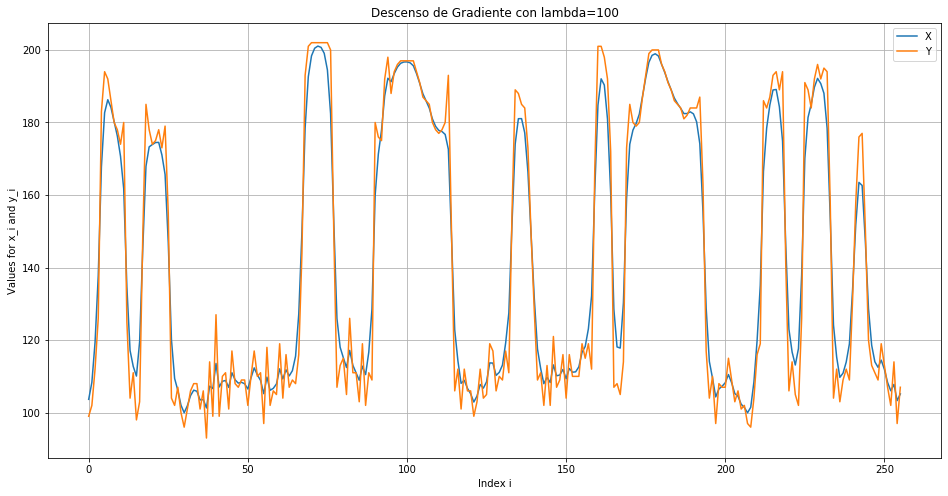
\includegraphics[scale=0.26]{dl1.png}}
	\caption{Obtención del minimizador para la función con $\lambda=1$, el suavizado de los la serie de los valores de Y es más intenso.}
	\label{figdl1}
\end{figure}

\begin{figure}[htbp]
	\centerline{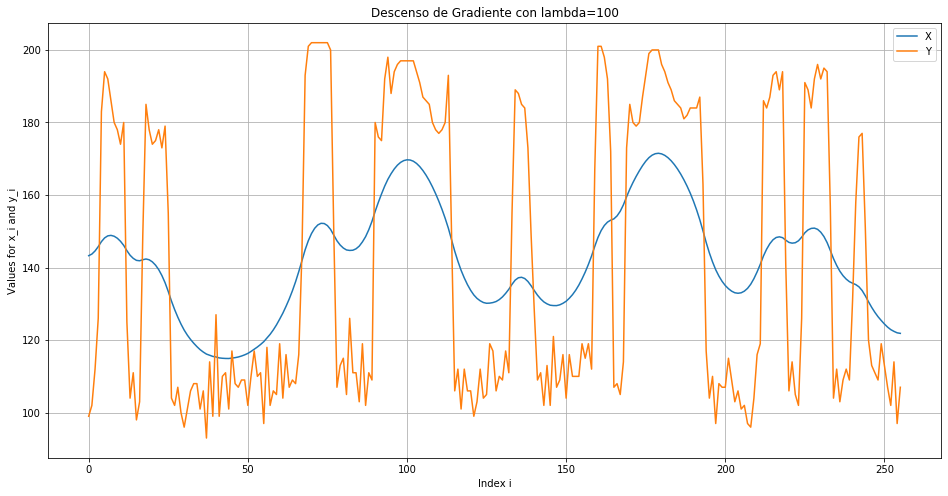
\includegraphics[scale=0.26]{dl100.png}}
	\caption{Obtención del minimizador para la función con $\lambda=100$, el suavizado de los la serie de los valores de Y es más intenso.}
	\label{figdl100}
\end{figure}

\begin{figure}[htbp]
	\centerline{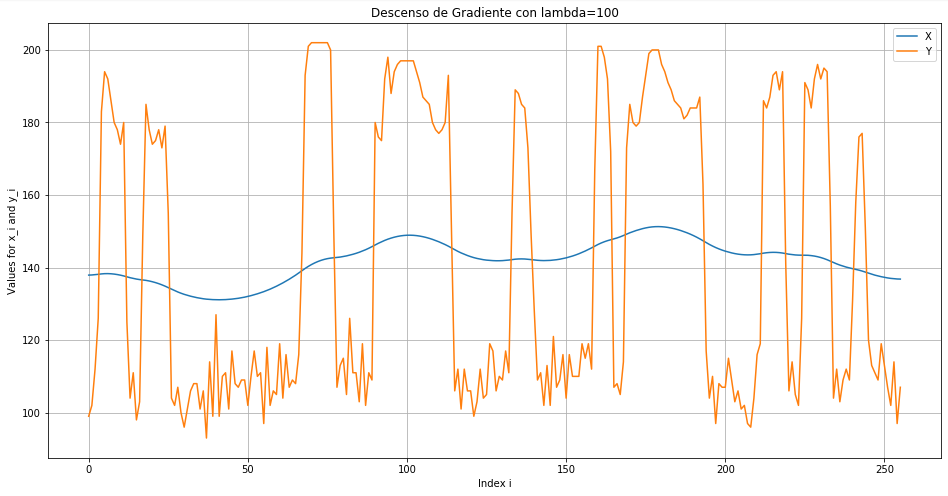
\includegraphics[scale=0.26]{dl1000.png}}
	\caption{Obtención del minimizador para la función con $\lambda=1000$, el suavizado de los la serie de los valores de Y es más intenso.}
	\label{figdl1000}
\end{figure}


\section*{}

\begin{thebibliography}{00}
\bibitem{b1} Jorge Nocedal, Stephen J. Wright, ``Numerical Optimization,'' Second Edition, Springer.
\end{thebibliography}

\end{document}
